\part{inter2ohdm}
\chapter{OHDM}
\section{Schema}
\begin{figure}[h]
	\caption{Schematischer Aufbau der OHDM Datenbank}
	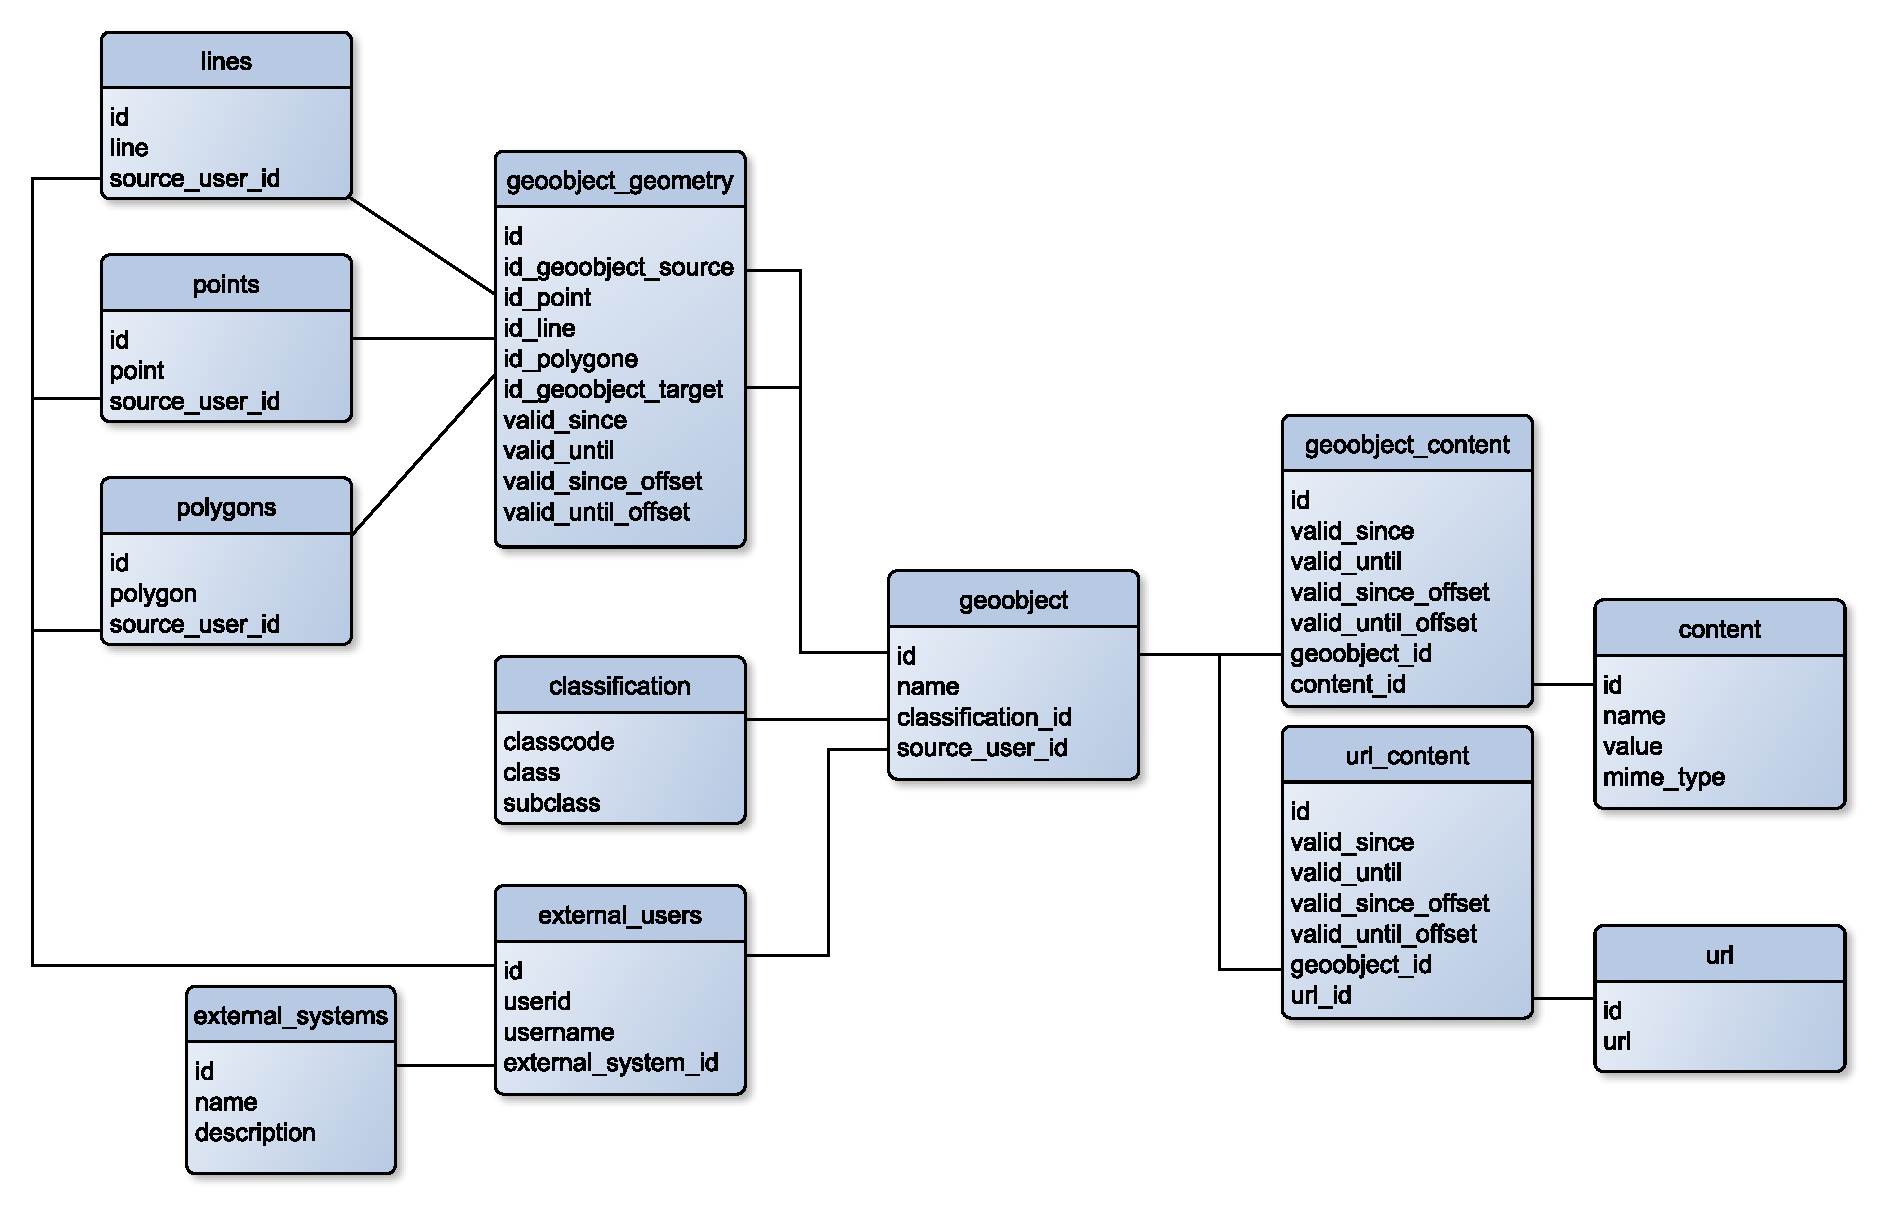
\includegraphics[width=\linewidth]{img/ohdm_datamodel.pdf}
\end{figure}
Die Erstellung des Schemas wurde mithilfe der existierenden Beschreibung von \\
\url{https://github.com/OpenHistoricalDataMap/OHDM-Documentation/wiki/OHDM-Data-Model} und den Konvertierten Einträgen des \gequote{alten} OHDMConverters realisiert.

\section{Theoretische Konvertierung}
\begin{figure}[h]
	\caption{Schematische Darstellung der einzelnen INSERT SQL Statemants}
	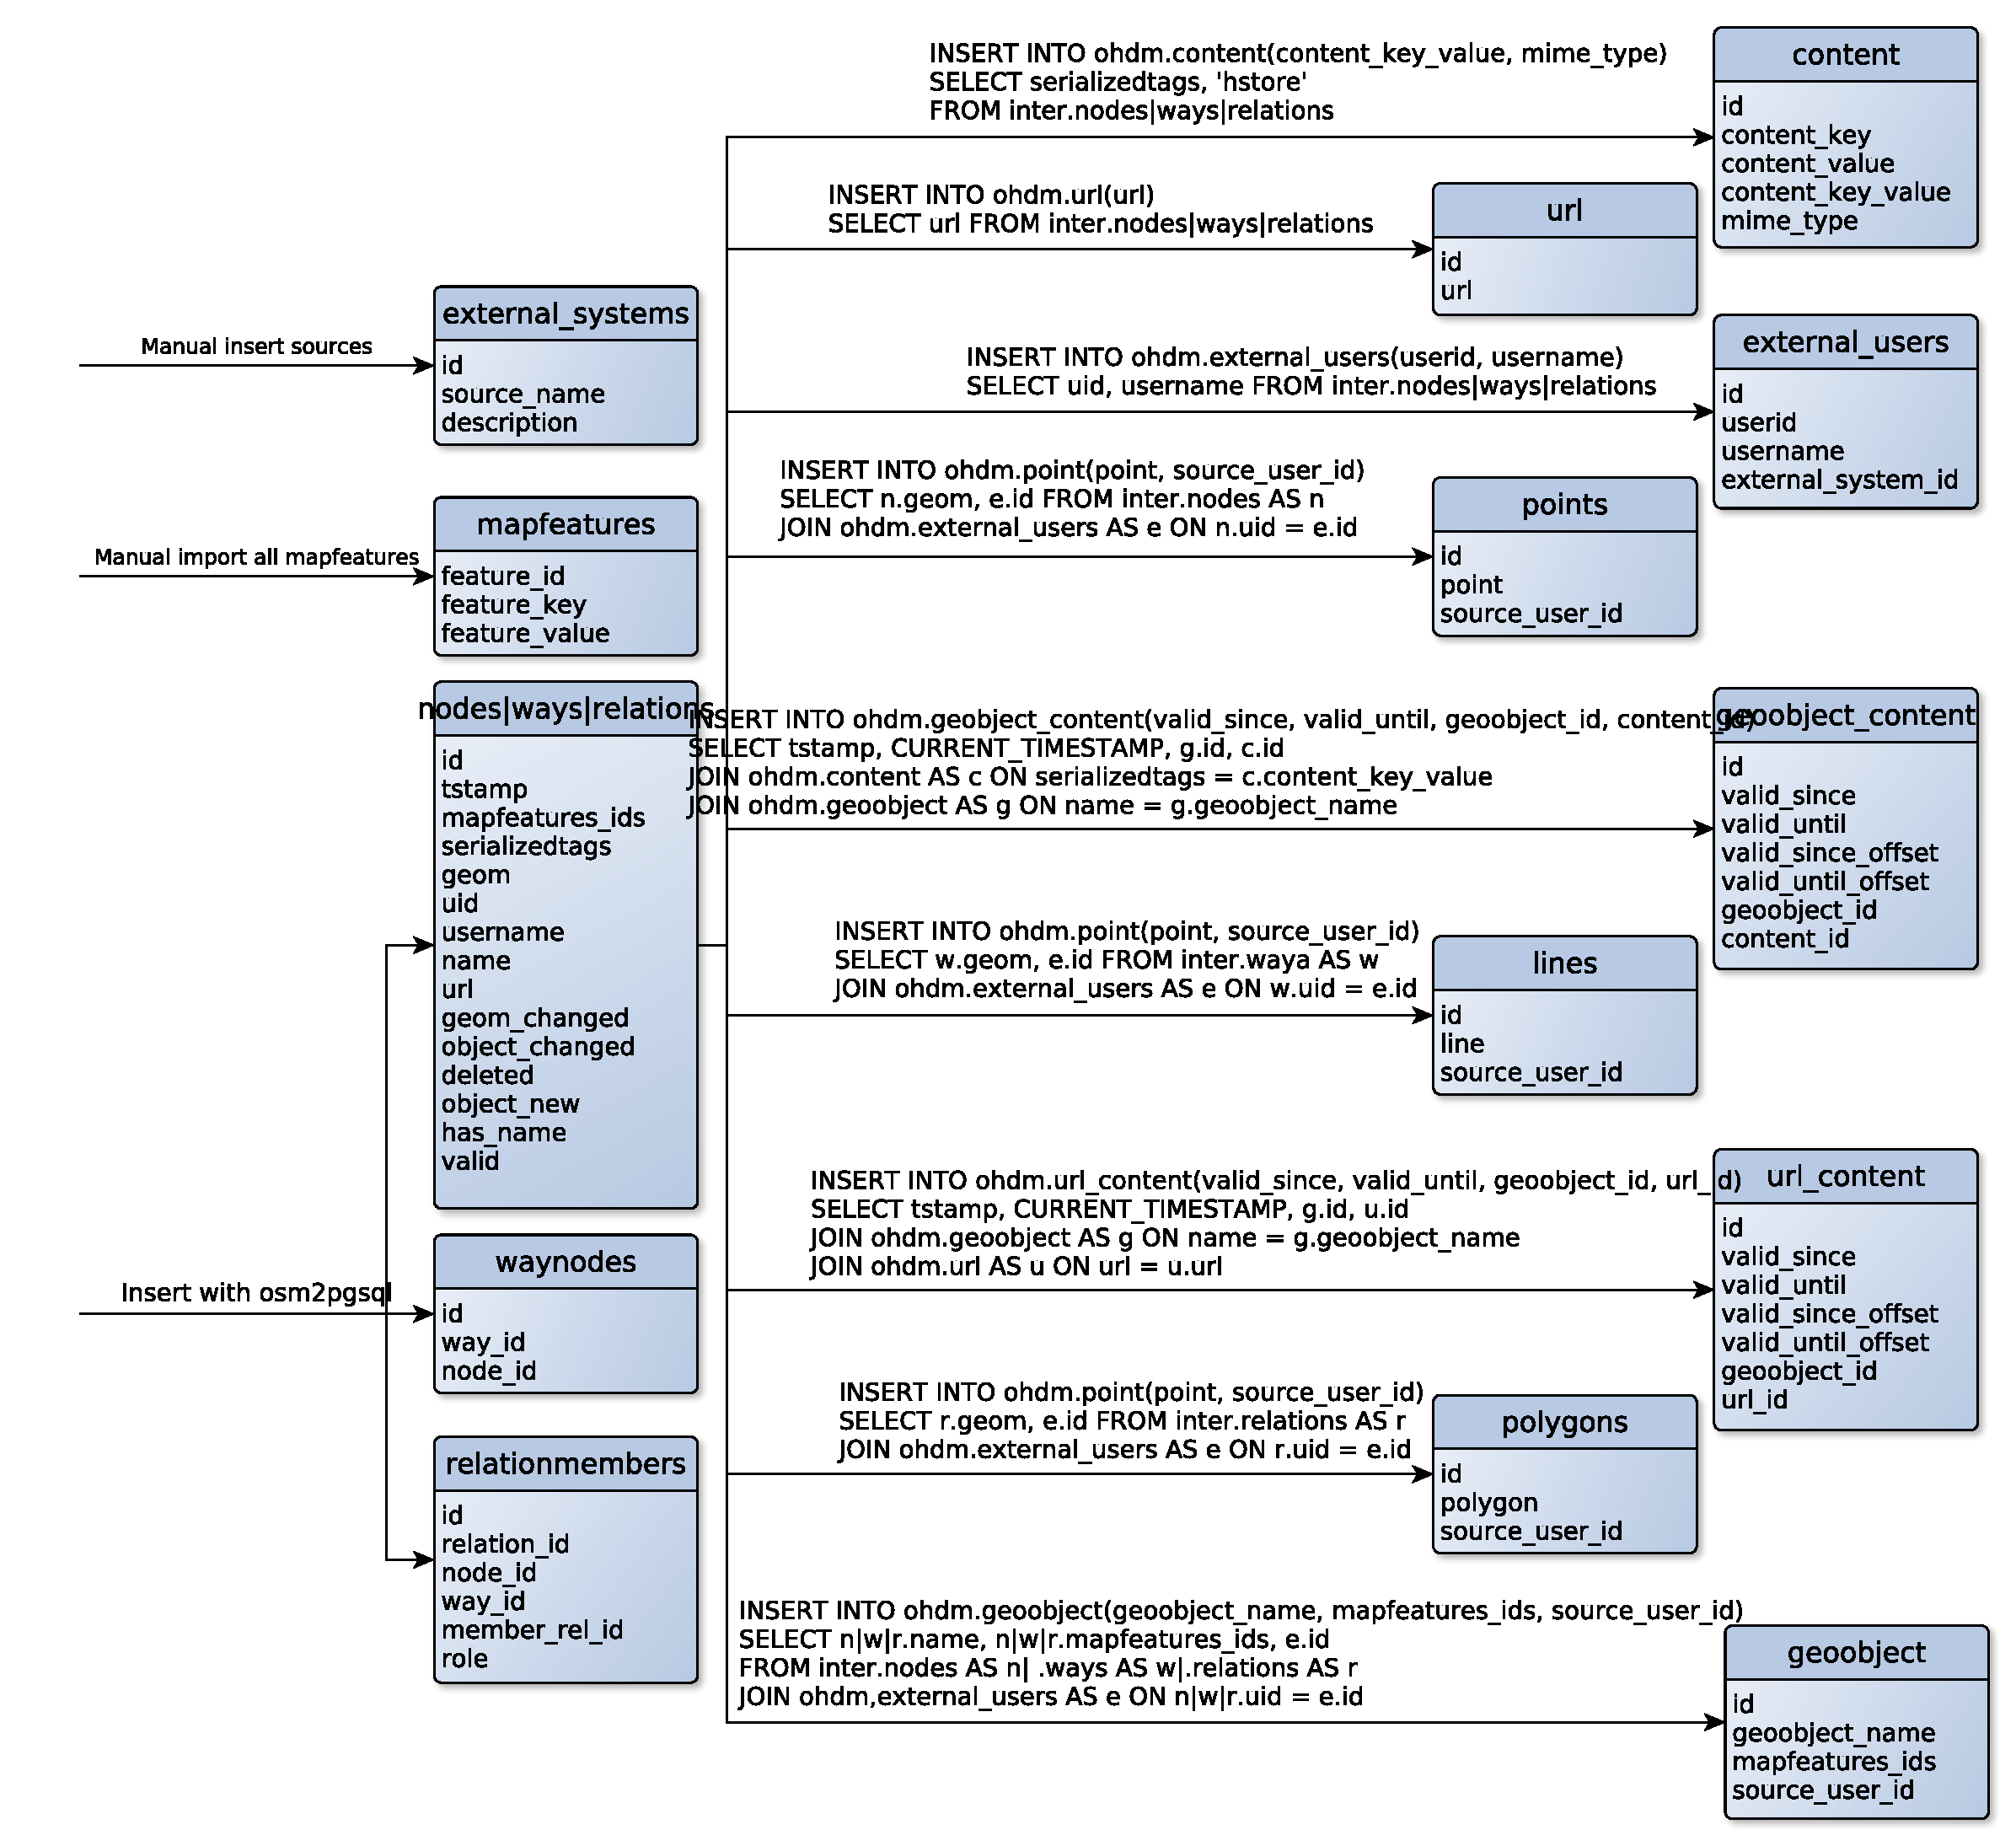
\includegraphics[width=\linewidth]{img/inter2ohdm_tableConvertionSchema1.pdf}
\end{figure}

\begin{figure}[h]
	\caption{Schematische Darstellung der einzelnen INSERT SQL Statemants}
	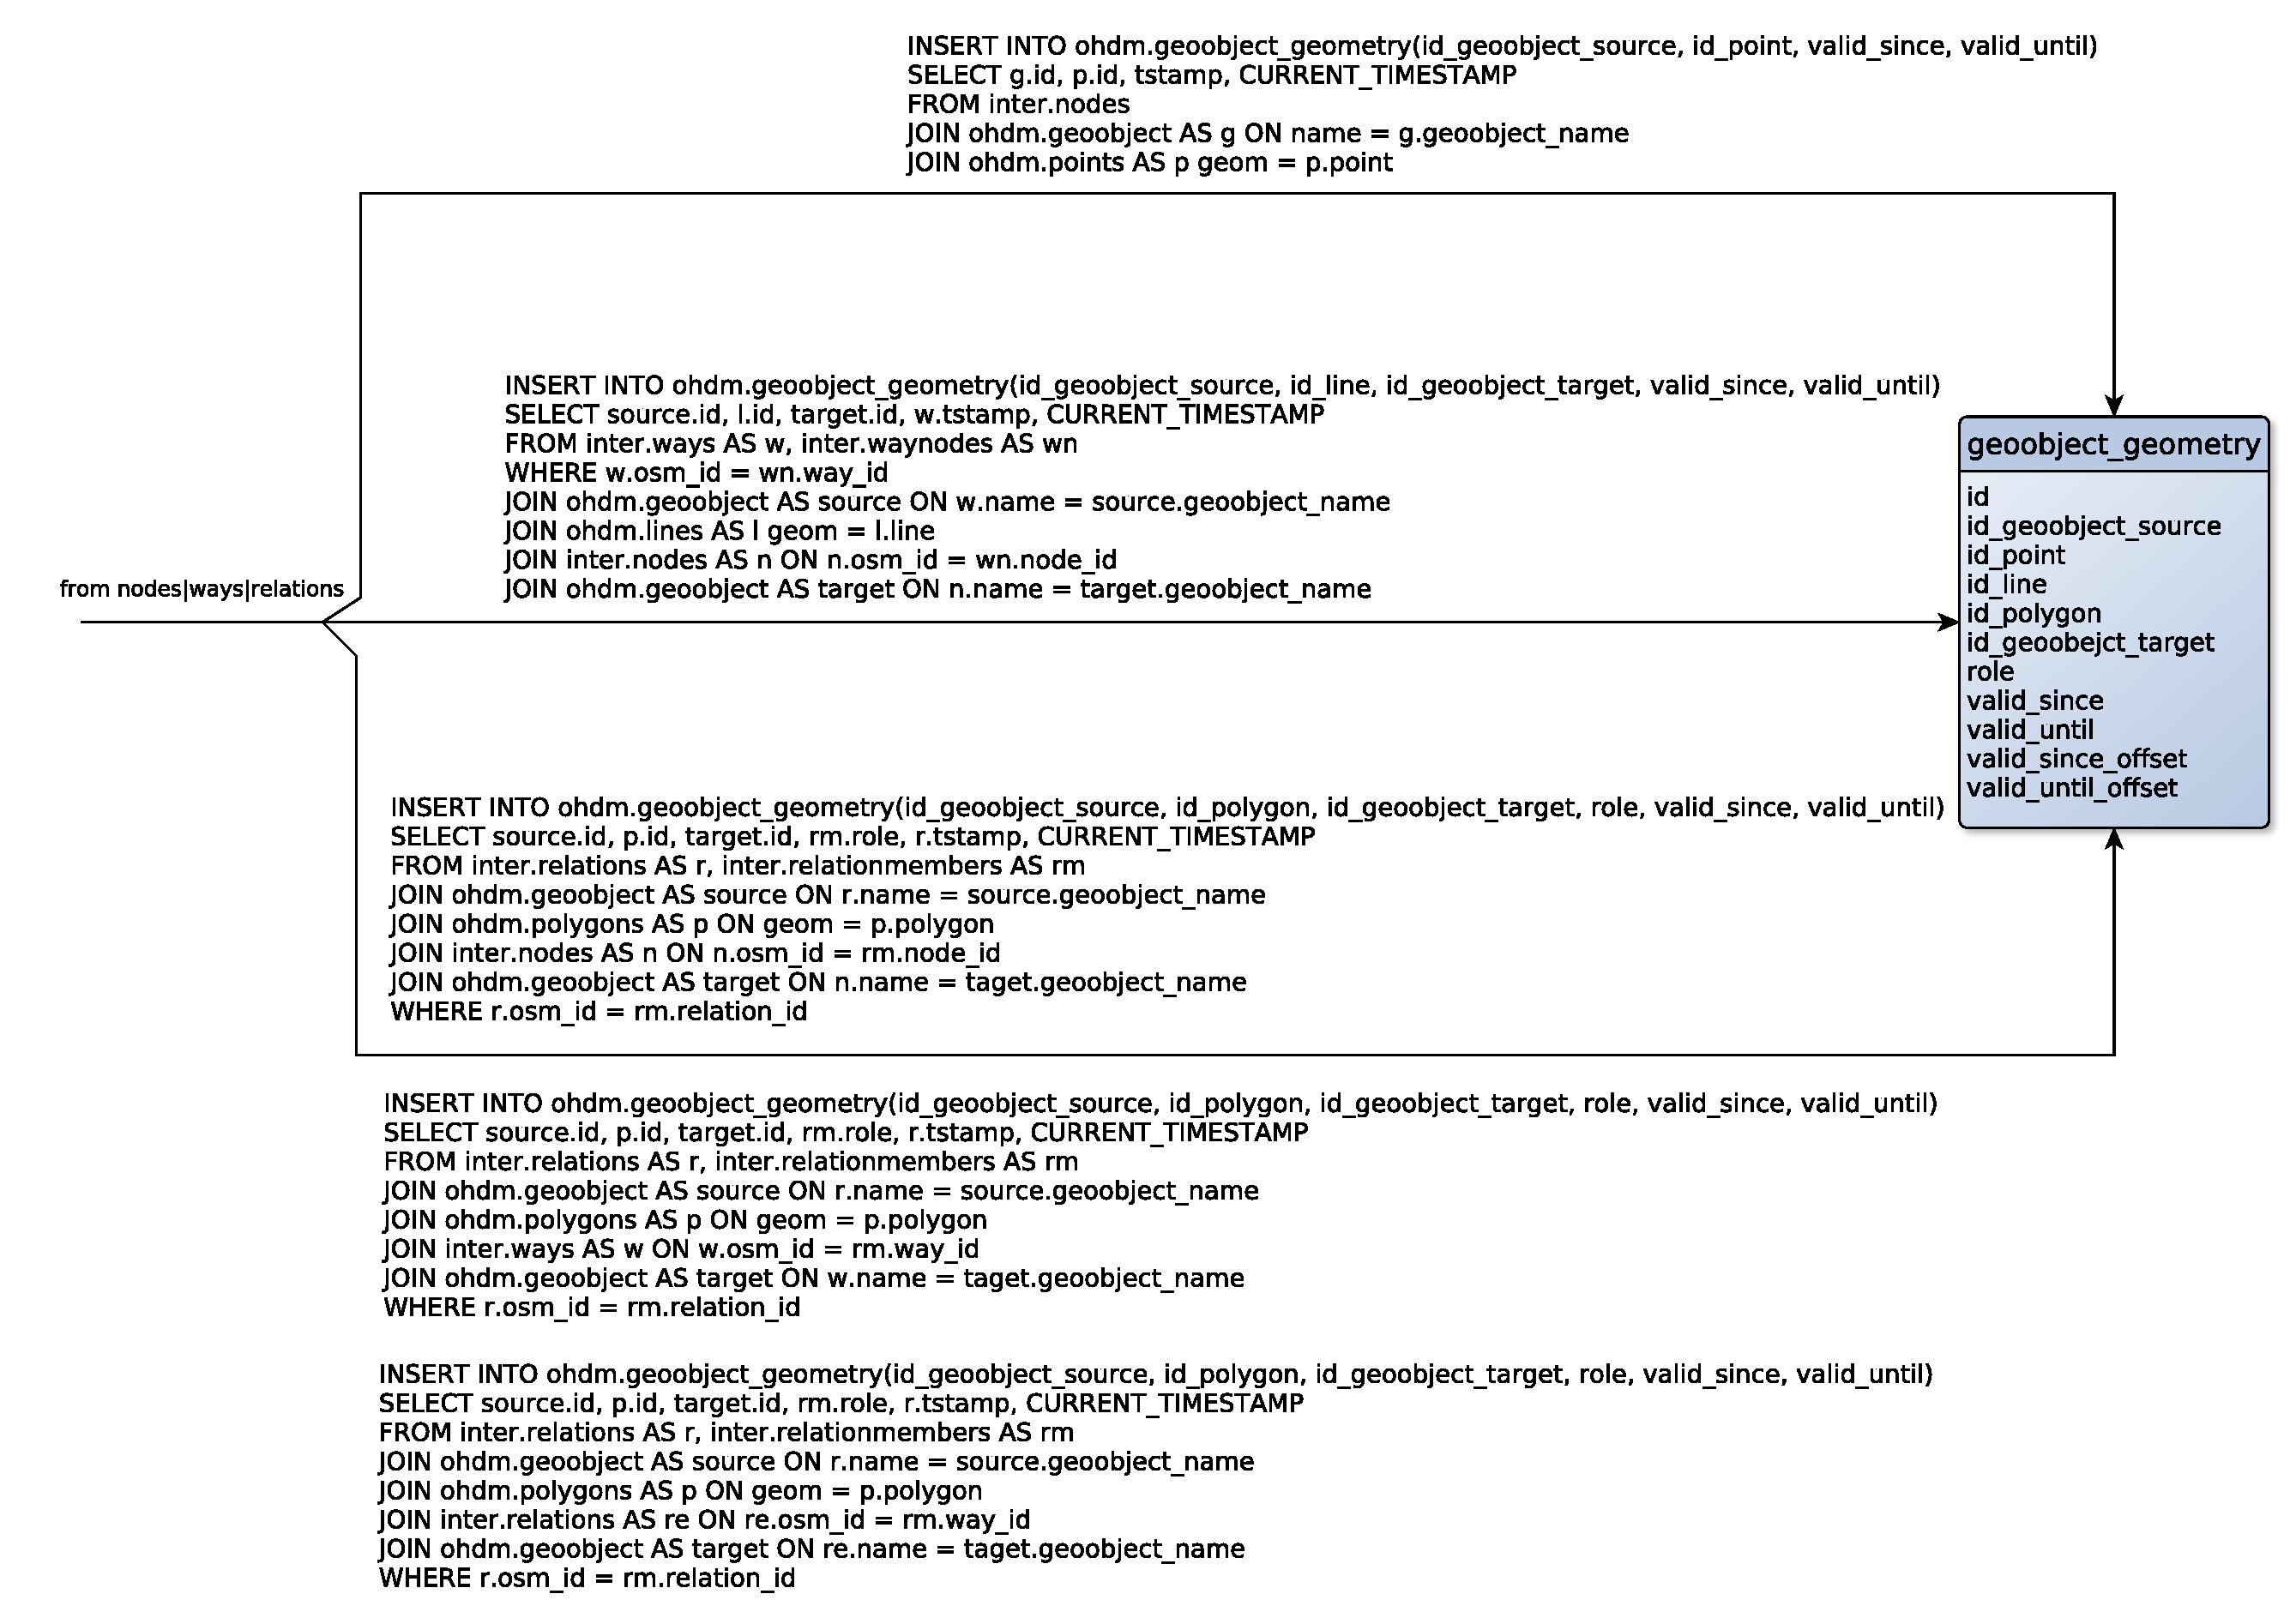
\includegraphics[width=\linewidth]{img/inter2ohdm_tableConvertionSchema2.pdf}
\end{figure}
